% Chapter 4

\chapter{Experimentación} % Main chapter title

\label{Chapter4} % For referencing the chapter elsewhere, use \ref{Chapter1} 

\lhead{Capítulo 5. \emph{Experimentación}} % This is for the header on each page - perhaps a shortened title

Este capítulo tiene por cometido presentar un conjunto de comparaciones experimentales entre los algoritmos descritos en los capítulos anteriores y dar conclusiones basadas en los datos empíricos recogidos de esta fase.\\
El alfabeto utilizado en los experimentos es \{a, c, g, t\}, donde estos símbolos representan las bases nitrogenadas adenina, citosina, guanina y timina respectivamente.\\
Ambos algoritmos presentan una fase de pre procesamiento en la cual se cargan los patrones en estructuras, las cuales son utilizadas para realizar la búsqueda, una fase de recorrida en la cual se recorre el texto procurando encontrar los patrones que sean de interés y finalmente, en el caso del algoritmo de MSW, se tiene una fase de post procesamiento, en la cual se realiza una recorrida en la estructura con el fin de obtener la cantidad de apariciones de cada patrón.\\
Por lo tanto, el número de patrones, el largo de los mismos y la cantidad total de caracteres del texto son variables que inciden en el rendimiento de estos algoritmos. Las mismas tienen un rol clave en la planificación de pruebas y en el análisis de los resultados.
\section{Ambiente y creación de pruebas}
Para la realización de las pruebas se utilizaron dos computadoras con diferentes prestaciones.
\begin{itemize}
\item MacBook Pro con sistema operativo OS X 10.8.5, procesador 2.5 GHz Intel Core i5 y memoria 4GB 1600MHz DDR3.
\item Laptop con sistema operativo Ubuntu 12.04, procesador Intel Celeron 575 2.0GHz y memoria de 2 GB 667MHz DDR2.
\end{itemize}
Se reiniciaron las computadoras antes de ejecutar las pruebas, esta acción es tomada con el fin de tener la memoria lo más limpia posible, con pocos procesos ejecuntandose en paralelo.\\
Se utilizaron los texto $\href{http://people.unipmn.it/manzini/dnacorpus/human/}{h2}$ \footnote{ $http://people.unipmn.it/manzini/dnacorpus/human/$}, $\href{ftp://ftp.ensembl.org/pub/release-67/fasta/canis_familiaris/}{Canis familiaris}$\footnote{ $ftp://ftp.ensembl.org/pub/release-67/fasta/canis_familiaris/$}, $\href{ftp://ftp.ensembl.org/pub/release-67/fasta/gallus_gallus/}{Gallus gallus}$\footnote{ $ftp://ftp.ensembl.org/pub/release-67/fasta/gallus_gallus/$}, $\href{ftp://ftp.ensembl.org/pub/release-67/fasta/anolis_carolinensis/}{Anolis}$\footnote{ $ftp://ftp.ensembl.org/pub/release-67/fasta/anolis_carolinensis/$} y $\href{ftp://ftp.ensembl.org/pub/release-67/fasta/homo_sapiens/}{Homo Sapiens}$\footnote{ $ftp://ftp.ensembl.org/pub/release-67/fasta/homo_sapiens/$}.
\begin{itemize}
\item h2 - Representa parte de la secuencia de ADN humano, tiene un tamaño aproximado de 236 MB, fue utilizado únicamente para generar patrones de prueba.
\item Canis - Representa la secuencia de ADN de un cromosoma de los perros domésticos, tiene un tamaño aproximado de 91 MB.
\item Anolis - Representa parte de la secuencia de ADN del reptíl Carolina (Anolis Carolinensis), tiene un tamaño aproximado de 75 MB.
\item Gallus - Representa parte de la secuencia de ADN del gallo, tiene un tamaño aproximado de 1.05 GB
\item Homo Sapiens - Representa parte de la secuencia de ADN del hombre, tiene un tamaño aproximado de 1.43 GB.
\end{itemize}
La mayoría de los \emph{textos} utilizados se encuentran codificados en formato {\bf FASTA} \cite{website:fasta}. Este formato comienza con una línea de descripción la cual es seguida por una secuencia de símbolos codificados en ASCII, donde cada símbolo representa una base nitrogenada según el estándar IUPAC \cite{website:iupac}. Dado que el programa espera un formato plano conteniendo únicamente los símbolos del alfabeto \{a, c, g, t\}, es necesario realizar una transformación de los \emph{textos}. Esta tarea se efectúa mediante el uso de un script de $\href{http://www.gnu.org/software/bash/manual/bashref.html}{Bash}$ \footnote{Referencia de Bash de GNU: $http://www.gnu.org/software/bash/manual/bashref.html$} ({\bf FastaCleaner.sh}) el cual se encarga de la conversión del formato FASTA a uno en que el texto final solo contenga simbolos del alfabeto \{a, c, g, t\}.\\
El conjunto de patrones que se requiere buscar es generado a partir de un texto; para ello se construyó un programa escrito en C++ ({\it BuildPatternSet.cpp}) que recibe como entrada la ruta al archivo que contiene el texto, la cantidad de patrones requerido y el largo de caracteres mínimo y máximo de cada patrón. La salida de dicho utilitario es un archivo conteniendo una secuencia de patrones (con la cantidad indicada). Los patrones son obtenidos de posiciones aleatorias del texto seleccionado y el largo de cada uno de ellos es un valor elegido al azar dentro del rango pre establecido por los valores mínimo y máximo ingresados.\\
Además de dicho generador se creó un script Bash ({\bf TestGenerator.sh}) que permite la creación de múltiples juegos de datos (utilizando el programa anteriormente mencionado), teniendo en cuenta los valores requeridos para cada prueba.\\
Los algoritmos analizados difieren en la forma en que leen los patrones, AC realiza la lectura en orden secuencial mientras que MSW lo hace de forma inversa. Con el fin de que la representación de los patrones no afecte la comparación experimental se creo un script Bash ({\bf PatInverse.sh}) que invierte cada uno de los patrones. De esta forma, cada prueba tendrá dos juegos de archivos, uno asignado a AC y otro, el inverso del primero, asignado a MSW.\\
Todas las pruebas se ejecutaron sobre un mismo programa (PDG), escrito en lenguaje C++, el cual cuenta con la posibilidad de configurar mediante argumentos el algoritmo a ejecutar, la ruta al archivo con los patrones a buscar, la ruta al texto a ser explorado, la cantidad de patrones a buscar, el tamaño de bloque de lectura y diferentes argumentos relativos a la salida. Puede encontrar más información relacionada con el programa principal en el cuadro \ref{table:PDG} del apéndice \ref{AppendixA}.\\
Cada prueba realizada tiene asociada un script de ejecución que ejecuta PDG con argumentos apropiados para el cometido de la prueba planificada. La salida de cada prueba es almacenada en archivos, los cuales son consolidados posteriormente en una única tabla con todos los valores de interés. Finalmente se transforma dicha grilla a un archivo con un formato apropiado para ser graficado por el programa $\href{http://www.gnuplot.info/}{Gnuplot}$ \footnote{ Sitio web de Gnuplot $www.gnuplot.info/$}. Para realizar las gráficas en Gnuplot se crea un conjunto de ejecutables Gnuplot (uno por cada juego de gráficas) que permiten tomar el archivo obtenido del proceso anteriormente descrito y obtener del mismo un conjunto de gráficas. También fueron utilizadas otras herramientas provistas por los sistemas operativos como {\bf time}, {\bf vmstat} y {\bf top}, las cuales fueron utilizadas para tomar medidas de consumo de memoria y de tiempo de ejecución.\\
Durante la construcción del programa se utilizó la herramienta {\it “Instruments”} provista por el IDE XCode (versión 4.x y 5.x) para medir el uso de memoria del aplicativo y encontrar posibles filtraciones de memoria.
\section{Medidas}
De los experimentos se extrae el tiempo de procesamiento y la memoria consumida como medidas a ser analizadas.
Definimos tiempo de procesamiento como el número total de segundos que el procesador le dedica al proceso de interés.
De la memoria consumida obtenemos dos valores, estos son: tamaño de memoria residente ({\textbf RSS} – {\it resident set size}) y el tamaño de la memoria virtual del proceso ({\textbf VSZ} – {\textit{virtual set size}).\\
El tiempo es medido a travéz de la función {\it clock} de {\it time.h}. Esta función retorna el número total de ticks de reloj consumidos por el proceso. Para obtener el tiempo total transcurrido en la ejecución de un fragmento de código, se inicializa al comienzo de la región de interés una variable de tipo clock\_t  con el valor retornado por {\it clock}, luego se invoca nuevamente a dicha función al final del código de interés, obteniéndose finalmente la diferencia entre ambos valores ($t_{final}$ - $t_{inicial}$). Dado que es de nuestro interés obtener el tiempo medido en segundos, debemos hacer un cambio de unidades (de ticks de reloj a segundos), este cambio lo realizamos dividiendo el resultado obtenido entre la constante {\bf CLOKS\_PER\_SEC}.\\
Por su lado, el consumo de memoria es medido de diferente forma, según el sistema operativo utilizado. En Ubuntu ejecutamos esta tarea através de la lectura del archivo alojado en /proc/self/stat. Este pseudo archivo de sistema presenta información pormenorizada del proceso, brindando, entre otros valores, datos detallados del consumo de memoria.  \\
En MacOs no se cuenta con el archivo de estado anteriormente mencionado, para realizar la medición en este sistema operativo se utiliza {\it mach.h}.
\section{Pre procesamiento}
\label{sec:pre_procesamiento}
Comenzamos analizando la evolución de los tiempos de ejecución y consumo de memoria de la etapa de pre procesamiento en ambos algoritmos.\\
Se presentan diferentes pruebas agrupadas en dos conjuntos que pretenden evaluar diferentes características de los algoritmos. Dichas agrupaciones son las siguientes:
\begin{enumerate}
\item Se utiliza una cantidad fija de patrones, variándose de forma incremental el largo de los mismos. Específicamente, cada prueba consta de n experimentos, donde los patrones del experimento número i, $1\le i\le n$, son de largo $k_{l} * i + L$; donde $k_{l}$ es una constante y $L$ es un número aleatorio sorteado uniformemente en el rango  [minLength, maxLength].
\item Se utilizan patrones de largo comprendidos en un entorno fijo, [minLength, maxLength], e incrementamos linealmente la cantidad de patrones con cada experimento. Por lo tanto, en el i-ésimo experimento usamos exactamente $k_{p} * i$ patrones, siendo $k_{p}$ una constante que determina la cantidad de patrones a incrementar.
\end{enumerate}
Como se detalló en el capítulo anterior, MSW debe construir una estructura que represente todos los sufijos de cada uno de los patrones, esto produce que el algoritmo cree un nodo por cada sufijo diferente que se encuentre en el conjunto de patrones. Por otro lado, AC crea un nuevo nodo $n_{i}$ asociado al carácter i-ésimo  de una palabra w si y solo si se tiene que $w_{1..i}$  no se encuentra dentro de la estructura.\\
Cada nodo de MSW debe almacenar la información necesaria para referenciar los nodos hijos y la subsecuencia que representa, además, por motivos de implementación debe mantener en memoria las transiciones junto con la estructuras necesarias para su creación como las referencia al nodo padre y sufijo.\\
Por contraparte, cada nodo de AC sólo almacena las referencias a los hijos, al nodo de referencia en caso de fallo y un arreglo de salidas, este último solo no será vacío en los casos en que el nodo represente el último carácter de algún patrón. Todo ello hace que, para juegos de patrones de largo grande, el tamaño de memoria que requiere el algoritmo AC tiende a ser sensiblemente más pequeño que en MSW. 
En las diversas pruebas realizadas se aprecia una notoria diferencia en el consumo de memoria entre ambos algoritmos, está diferencia es más acentuada cuando se analizan juegos con patrones suficientemente largos. \\
Para los casos en que se tiene múltiples patrones con largo lo suficientemente pequeños, MSW sigue consumiendo más memoria, pero la diferencia entre ambos algoritmos es inferior que en la situación anterior. Esto se debe a que, para patrones largos, MSW tiene un costo de almacenamiento (y cómputo) alto ya que debe crear una cantidad apreciable de nodos de sufijo. \\
El cuadro \ref{tab:Definicion_Pruebas} presenta cuatro pruebas, dos para cada agrupación definida anteriormente. Los resultados de las dos primeras pruebas serán estudiados en esta y en la siguiente sección, mientras que el efecto de las últimas dos pruebas sobre los algoritmos serán abarcados en la sección \ref{sec:procesamiento}.
\begin{table}[H]
\begin{center}
\begin{tabular}{ | l | l | l | l | l | l | l |}
\hline
    Prueba & Experimentos & Nro Patrones & MinLength & MaxLength & $k_{l}$ & $k_{p}$ \\ \hline
    1 & 50 & $k_{p} * i + L$ & 30 & 40 & - & 8.000 \\ \hline
    2 & 50 & 50 & 10.000 + $k_{l} * i$ & 11.000 + $k_{l} * i$ & 5.000 & - \\ \hline
    3 & 400 & $k_{p} * i + L$ & 10 & 20 & - & 10 \\ \hline
    4 & 400 & 10 & 10 + $k_{l} * i$ & 20 + $k_{l} * i$ & 20 & - \\ \hline
\end{tabular}
\captionof{table}{Pruebas realizadas sobre los algoritmos AC y MSW} \label{tab:Definicion_Pruebas} 
\end{center}
\end{table}
Luego de ejecutar las dos primeras pruebas se obtiene el gráfico de la figura \ref{fig:Memoria50PatsVsMultiPats} que muestra el comportamiento de la fase de pre procesamiento expuesto anteriormente. Las gráficas AC\_Test1\_Mem y MSW\_Test1\_Mem representan la evolución del consumo de memoria de AC y MSW para la prueba 1, respectivamente, mientras que  AC\_Test2\_Mem y MSW\_Test2\_Mem representan la evolución del consumo de memoria para la prueba 2 de los algoritmos de AC y MSW respectivamente. \\
A modo de ejemplo, si tomamos como referencia 1.2\e{7} caracteres totales de patrones, se tiene para la prueba 2 una diferencia cercana a 500MB entre las ejecuciones de MSW y AC; por otro lado, en mismas condiciones, se tiene que la prueba 1 la diferencia se achica a valores del entorno de 120MB.\\
\begin{figure}[H]
	\centering
		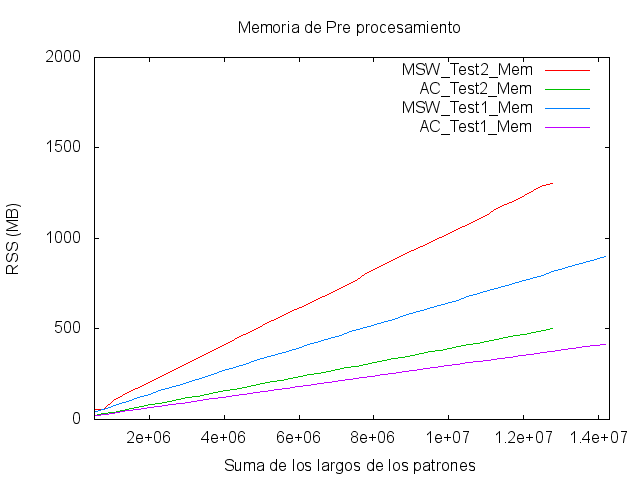
\includegraphics[scale=0.5]{Ubuntu_50PatsVsMultiPats_preprocesamiento.png}
		\rule{35em}{0.5pt}
	\caption[gráfica RSS]{Memoria residente (RSS en Ubuntu)}
	\label{fig:Memoria50PatsVsMultiPats}
\end{figure}
En ambos algoritmos, el tiempo de ejecución del pre procesamiento es lineal en la suma de los largos de los patrones. Sin embargo, en la práctica, se requiere más tiempo de ejecución por parte de MSW que por AC. \\
En ambos casos, los patrones son cargados en una estructura inicial.
La construcción de la clausura FSM a partir de la estructura inicial (GCT) requiere de varios ciclos de ejecución recursiva para llevar a cabo la transformación de la estructura, dentro de los cuales pueden realizarse modificaciones de los nodos existentes y creaciones de nuevos nodos. Por otro lado el algoritmo requiere una etapa final en la cual se realiza la propagación de las transiciones, esta operativa requiere recorrer toda la GCT. Mientras tanto, AC, luego de cargar la estructura básica en memoria no necesita insertar más nodos. Este algoritmo recorre una única vez su estructura agregando elementos al conjunto {\it “output”} y generando la función de fallos en forma iterativa.
Resulta entonces que MSW debe realizar una operativa más compleja en la fase de pre procesamiento que AC.\\
Por esta razón, es esperable, y así fue confirmado experimentalmente, que en la fase de pre procesamiento se obtengan tiempos de ejecución mayores por parte de MSW que de AC.\\
La gráfica \ref{fig:Tiempo50PatsVsMultiPats} presenta el tiempo total de la fase de pre procesamiento para diferentes pruebas. En el eje de las abscisas se presenta el largo total de caracteres procesados, mientras que en el eje Y se muestra el tiempo medido en segundos. Los gráficos AC\_Test1\_T y MSW\_Test1\_T corresponden a la medición del tiempo de pre procesamiento de la prueba 1 para los algoritmos AC y MSW respectivamente, mientras que AC\_Test2\_T y MSW\_Test2\_T presenta los gráficos para la prueba 2.\\
De esta representación observamos que los tiempos evolucionan linealmente en todos los casos, no obstante, a igual cantidad de caracteres total del archivo de patrones, MSW tarda más en procesar patrones suficientemente largos que muchos cortos. Un comportamiento inverso tiene AC, este algoritmo tarda más en procesar un conjunto considerable de patrones (con largo chico) que en realizar la misma tarea con pocos patrones de largo considerable (en relación a consideraciones de MSW).\\
Comparativamente AC es más veloz que MSW en las dos configuraciones pero cabe destacar que para la prueba 1 la diferencia máxima es del entorno de 12 segundos mientras que la diferencia máxima en la prueba 2 es más de 12 segundos\\
Pruebas similares, con otras configuraciones de cantidad de patrones fijo y rangos de largo fijo arrojaron tendencias similares al ser ejecutadas en los dos ordenadores de prueba.\\
\begin{figure}[htbp]
	\centering
		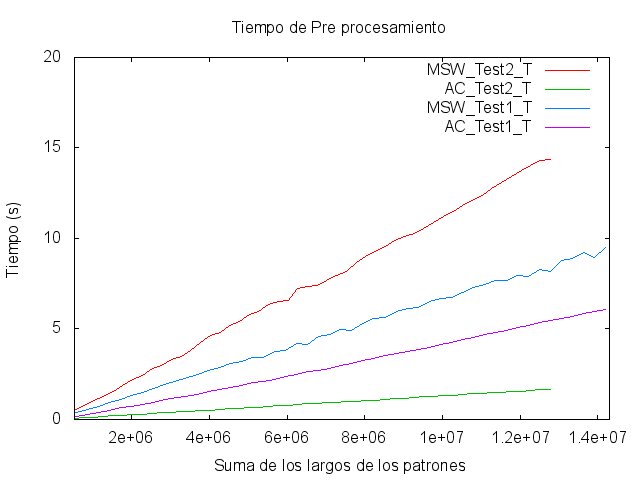
\includegraphics[scale=0.5]{Ubuntu_50PatsVsMultiPats_preprocesamiento_tiempo.png}
		\rule{35em}{0.5pt}
	\caption[gráfica tiempo de ejecución de pre procesamiento]{Tiempo de ejecución de pre procesamiento (medido en Ubuntu)}
	\label{fig:Tiempo50PatsVsMultiPats}
\end{figure}
\section{Procesamiento sobre textos}
\label{sec:procesamiento}
En la sección anterior analizamos los algoritmos en la etapa de pre procesamiento. Dicha fase genera las estructuras de datos necesarias para realizar la búsqueda del conjunto de patrones sobre el texto contenido en un archivo.\\
El archivo de texto es leído de disco a memoria secuencialmente en bloques de tamaño fijo. Cada uno de los bloques es procesado cáracter a cáracter por el programa principal en ambos algoritmos. El procedimiento por el cual se realiza la lectura de cada archivo es compartido por ambos algoritmos, de modo que los costos de cómputo y consumo de memoria  asociados a esta tarea son idénticos en ambos casos. 
Los algoritmos registran los hallazgos de correspondencia entre una secuencia de caracteres leída y los patrones que se están buscando. A partir de los datos registrados el programa puede generar un informe de la búsqueda al finalizar la recorrida sobre el texto. En nuestras pruebas, este informe consiste en la cantidad de veces que fue hallado cada uno de los patrones. En el caso de MSW, la información persistida no es suficiente, ya que, como se vió en el capítulo \ref{Chapter3}, es necesario realizar un post procesamiento para obtener los resultados finales.\\
Como se explicó en el capítulo \ref{Chapter3}, es posible liberar parte de la memoria utilizada por el algoritmo MSW luego de la fase de pre procesamiento. Sin embargo, dicha liberación no fue implementada en este proyecto. Dado que el procesamiento sobre el texto se realiza en bloques de tamaño fijo, el consumo global de memoria queda esencialmente determinada por la etapa de pre procesamiento.
Por esta razón, se considera un conjunto de pruebas que tienen como fin examinar los tiempos de ejecución de ambos algoritmos en la fase de procesamiento del texto y omitimos la evaluación del consumo de memoria en esta etapa.
Estos conjuntos son examinados contra los diferentes texto de prueba, tomando los tiempos de procesamiento del texto (recorrida y hallazgo de los múltiples patrones). 

\subsection{Efecto del conjunto de patrones sobre el tiempo de procesamiento de texto}
Al igual que en la sección \ref{sec:pre_procesamiento}, analizamos el comportamiento de los algoritmos ante variaciones en el largo y la cantidad de patrones. Se ejecutaron las cuatro pruebas especificadas en el cuadro \ref{tab:Definicion_Pruebas}, cada una de ellas sobre cuatro \emph{textos} diferentes. En estas pruebas se midió el tiempo de procesamiento de cada texto completo, omitiéndose el tiempo de pre y post procesamiento.
Comenzamos presentando las gráficas de la figura \ref{fig:Prueba1Tab}, correspondientes a la ejecución de la prueba 1 sobre los \emph{textos} de prueba. Observamos en las mismas que AC presenta una ventaja en relación a MSW hasta cierto punto, a partir del cual, MSW se mantiene por debajo de la curva de AC. 
\begin{figure}[H]
\centering
	\subfigure[Anolis]{%
	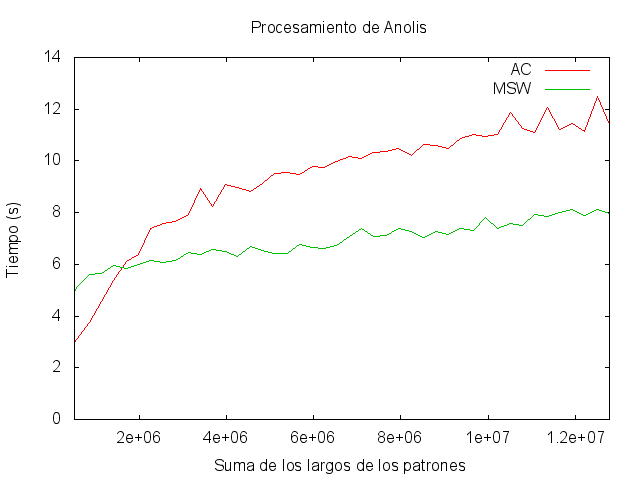
\includegraphics[scale=0.4]{Maci5_Procesamiento_Test1_Anolis.png}
	\label{fig:Prueba1Tab_a}}
\quad
	\subfigure[Canis]{%
	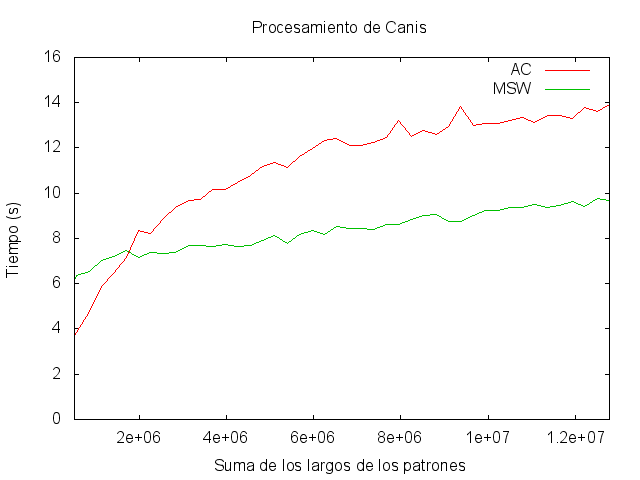
\includegraphics[scale=0.4]{Maci5_Procesamiento_Test1_Canis.png}
	\label{fig:Prueba1Tab_b}}
\quad
	\subfigure[Gallus]{%
	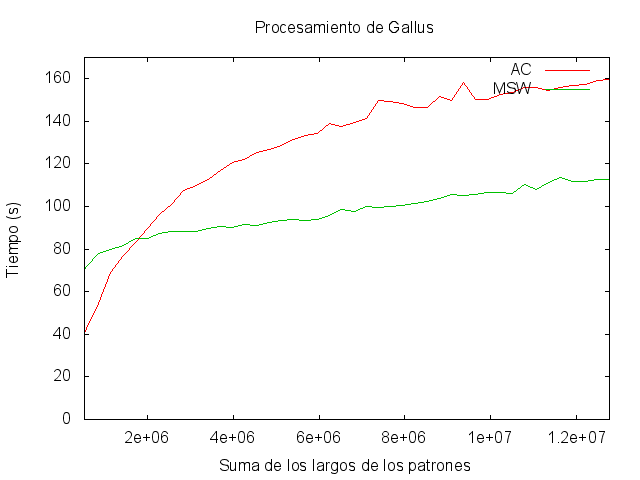
\includegraphics[scale=0.4]{Maci5_Procesamiento_Test1_Gallus.png}
	\label{fig:Prueba1Tab_c}}
\quad
	\subfigure[Homo Sapiens]{%
	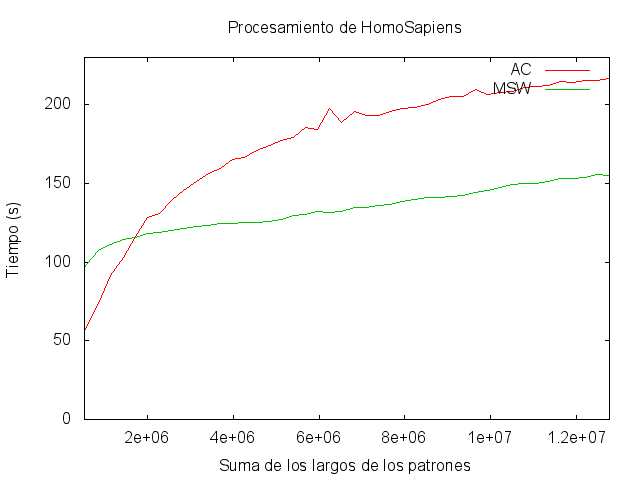
\includegraphics[scale=0.4]{Maci5_Procesamiento_Test1_HomoSapiens.png}
	\label{fig:Prueba1Tab_d}}
\caption{Tiempos de procesamiento de la prueba 1 (medido en Mac)}
\label{fig:Prueba1Tab}
\end{figure}
Cabe destacar que la prueba 1 puede contener hasta 400.000 patrones de largo corto, factor que afecta a AC, ya que aumenta la probabilidad de encontrar patrones dentro de los \emph{textos} de prueba (ver introducción del capítulo \ref{Chapter2}). Este hecho, mitiga la ventaja en consumo de memoria que tiene AC sobre MSW.
Por contra parte, al analizar las gráficas presentadas en la figura \ref{fig:Prueba2Tab}, correspondientes a la prueba 2, observamos que AC se mantiene casi constante mientras MSW es siempre creciente. 
\begin{figure}[H]
\centering
	\subfigure[Anolis]{%
	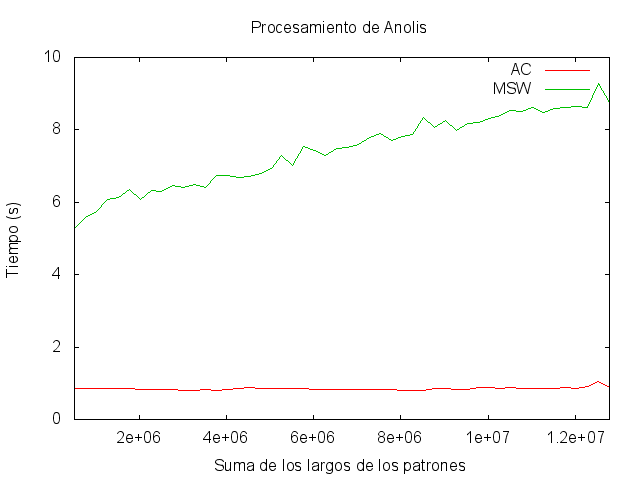
\includegraphics[scale=0.4]{Maci5_Procesamiento_10PatsCortos_Anolis.png}
	\label{fig:Prueba2Tab_a}}
\quad
	\subfigure[Canis]{%
	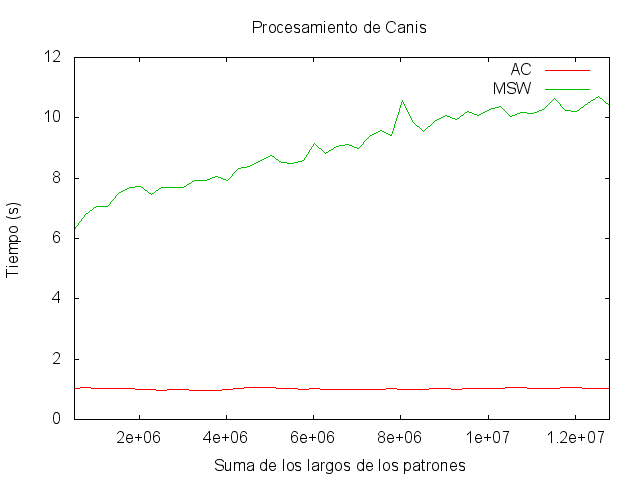
\includegraphics[scale=0.4]{Maci5_Procesamiento_10PatsCortos_Canis.png}
	\label{fig:Prueba2Tab_b}}
\quad
	\subfigure[Gallus]{%
	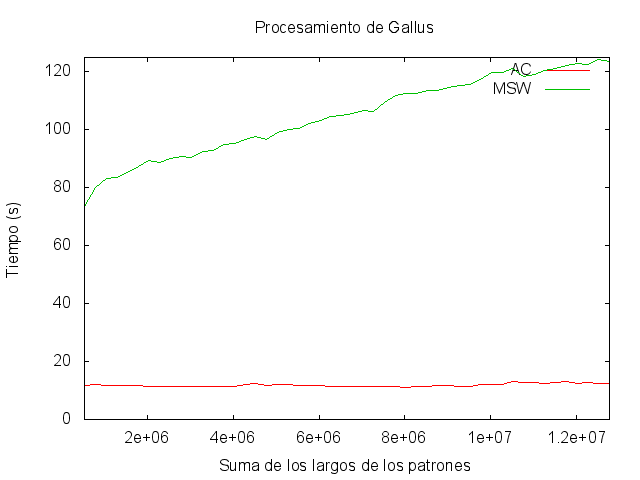
\includegraphics[scale=0.4]{Maci5_Procesamiento_10PatsCortos_Gallus.png}
	\label{fig:Prueba2Tab_c}}
\quad
	\subfigure[Homo Sapiens]{%
	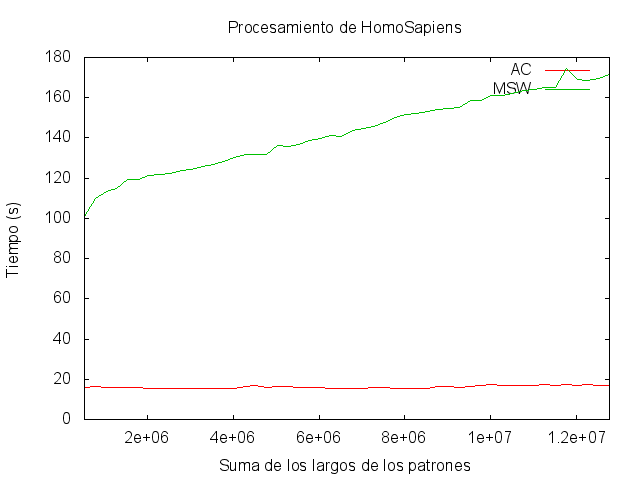
\includegraphics[scale=0.4]{Maci5_Procesamiento_10PatsCortos_HomoSapiens.png}
	\label{fig:Prueba2Tab_d}}
\caption{Tiempos de procesamiento de la prueba 2 (medido en Mac)}
\label{fig:Prueba2Tab}
\end{figure}
Los resultados de la prueba 3, presentados en la figura \ref{fig:Prueba3Tab}, se observa una clara ventaja de MSW sobre AC. La configuración usada en esta prueba es similar a la de la prueba 1, solo que el largo y la cantidad de patrones utilizada es mucho más pequeña que en la prueba 1.
\begin{figure}[H]
\centering
	\subfigure[Anolis]{%
	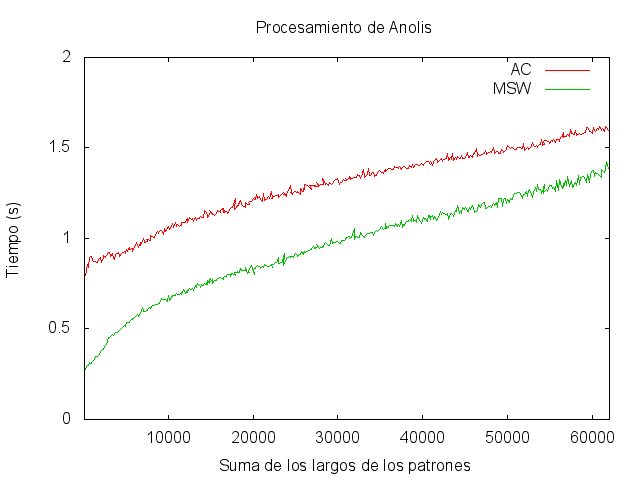
\includegraphics[scale=0.4]{Maci5_PequenosPatrones_Anolis.png}
	\label{fig:Prueba3Tab_a}}
\quad
	\subfigure[Canis]{%
	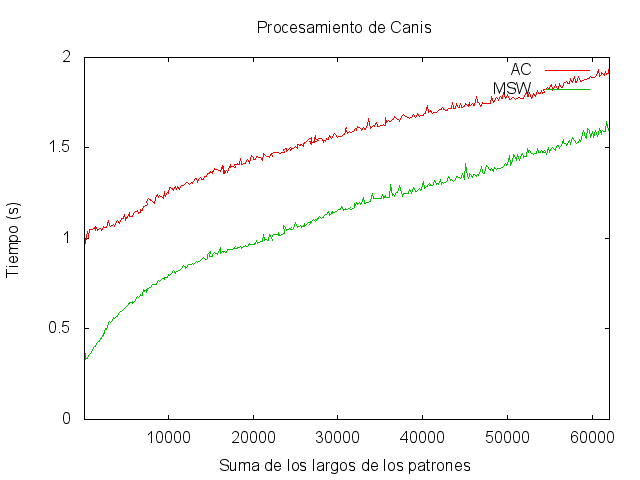
\includegraphics[scale=0.4]{Maci5_PequenosPatrones_Canis.png}
	\label{fig:Prueba3Tab_b}}
\quad
	\subfigure[Gallus]{%
	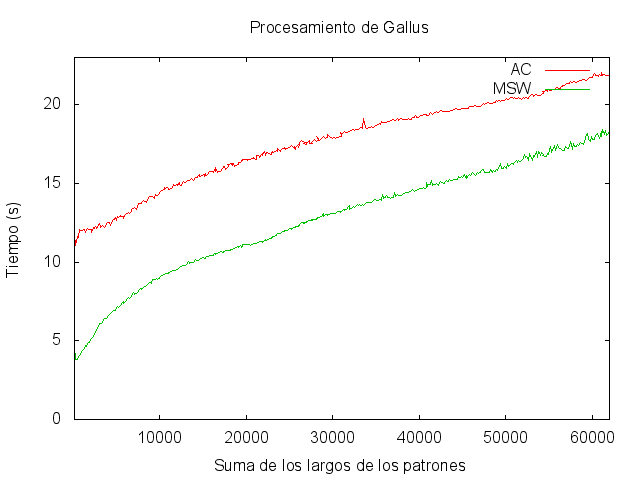
\includegraphics[scale=0.4]{Maci5_PequenosPatrones_Gallus.png}
	\label{fig:Prueba3Tab_c}}
\quad
	\subfigure[Homo Sapiens]{%
	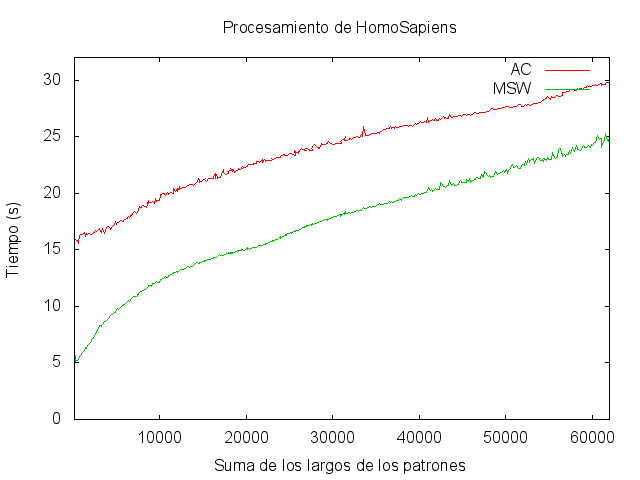
\includegraphics[scale=0.4]{Maci5_PequenosPatrones_HomoSapiens.png}
	\label{fig:Prueba3Tab_d}}
\caption{Tiempos de procesamiento de la prueba 3 (medido en Mac)}
\label{fig:Prueba3Tab}
\end{figure}
Al igual que en la prueba 2, los resultados de la prueba 4, presentados en la figura \ref{fig:Prueba4Tab}, muestran que los tiempos de procesamiento de AC tienen un comportamiento casi constante, mientras que para MSW la misma curva es siempre creciente. En el caso de la prueba 4 se tiene que, a partir de una cantidad de caracteres (suma total) de patrones, AC obtiene mejores tiempos de ejecución que MSW. En la prueba 2, por tratarse de muestras con largo total de caracteres varias unidades mayores que las usadas en la prueba 4, la curva descrita por MSW siempre se muestra por encima de la de AC.
\begin{figure}[H]
\centering
	\subfigure[Anolis]{%
	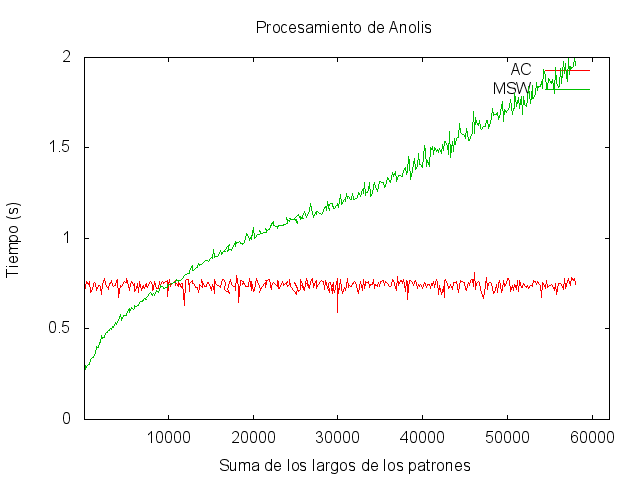
\includegraphics[scale=0.4]{Maci5_10PatsCortos_Anolis.png}
	\label{fig:Prueba4Tab_a}}
\quad
	\subfigure[Canis]{%
	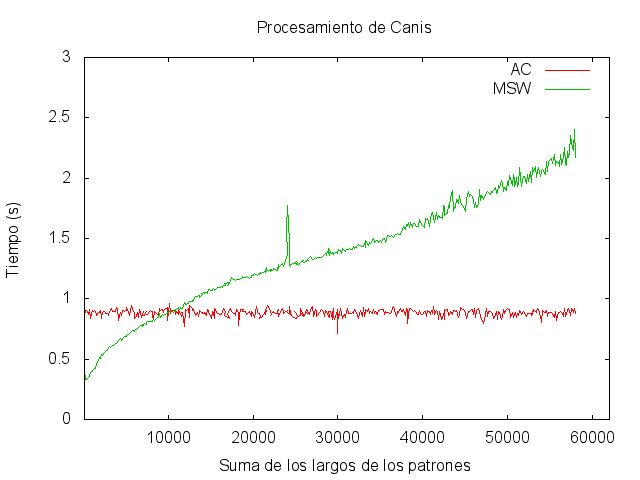
\includegraphics[scale=0.4]{Maci5_10PatsCortos_Canis.png}
	\label{fig:Prueba4Tab_b}}
\quad
	\subfigure[Gallus]{%
	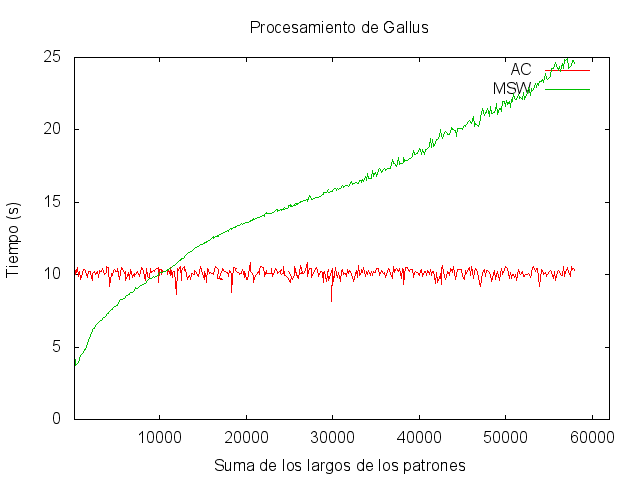
\includegraphics[scale=0.4]{Maci5_10PatsCortos_Gallus.png}
	\label{fig:Prueba4Tab_c}}
\quad
	\subfigure[Homo Sapiens]{%
	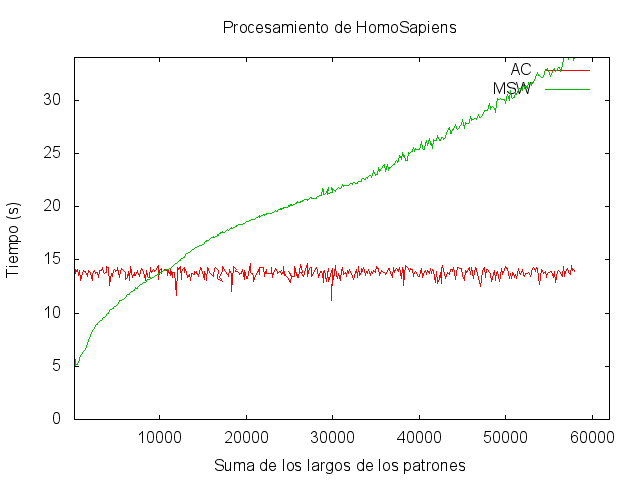
\includegraphics[scale=0.4]{Maci5_10PatsCortos_HomoSapiens.png}
	\label{fig:Prueba4Tab_d}}
\caption{Tiempos de procesamiento de la prueba 4 (medido en Mac)}
\label{fig:Prueba4Tab}
\end{figure}
A pesar de tener una cantidad total de caracteres de patrones similares a la prueba 4, la prueba 3 arroja diferentes resultados (esto también sucede si comparamos las pruebas 1 y 2). Esta comparación muestra que al variar el largo y la cantidad de patrones (conservando la suma de los caracteres) se obtienen diferencias entre estos algoritmos.
A pesar de que la segunda etapa de MSW es más sencilla que la de AC, lo cual haría esperar que fuera más eficiente es posible encontrar configuraciones en las cuales el tiempo de ejecución de la segunda etapa de MSW es mayor que la de  AC.
La figura \ref{fig:exp2_2Tab} resume estas observaciones.
\begin{figure}[H]

\centering
	\subfigure[Prueba 1]{%
	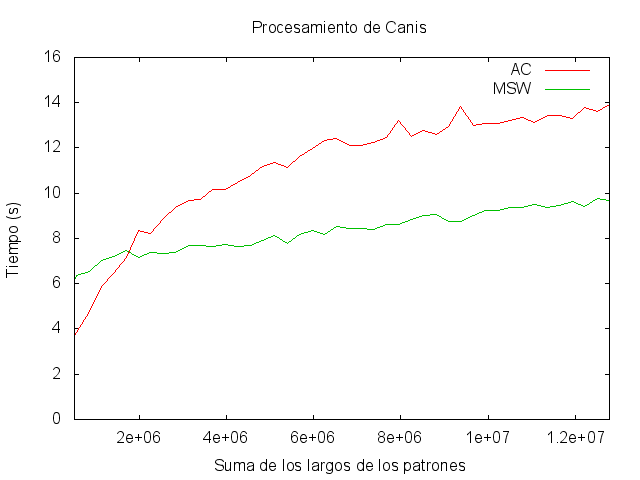
\includegraphics[scale=0.4]{Maci5_Procesamiento_Test1_Canis.png}
	\label{fig:exp2_2Tab_a}}
\quad
	\subfigure[Prueba 2]{%
	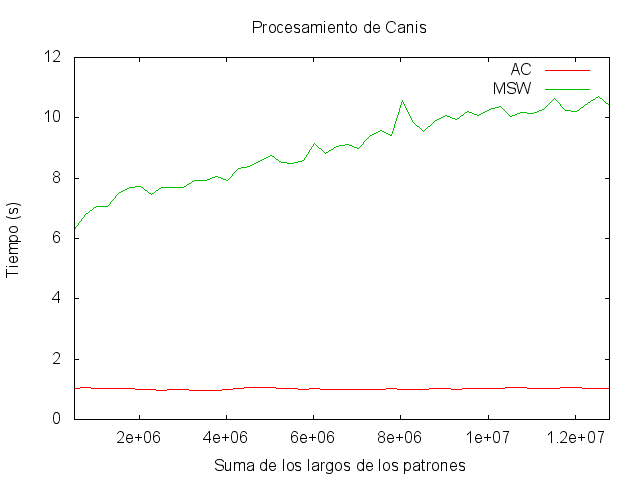
\includegraphics[scale=0.4]{Maci5_Procesamiento_10PatsCortos_Canis.png}
	\label{fig:exp2_2Tab_b}}
\quad
	\subfigure[Prueba 3]{%
	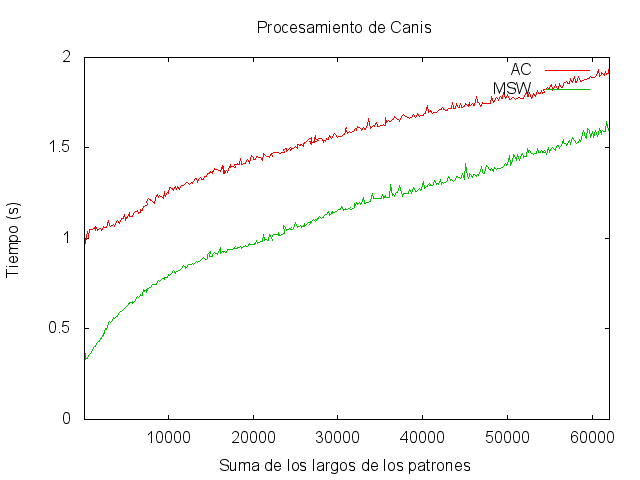
\includegraphics[scale=0.4]{Maci5_PequenosPatrones_Canis.png}
	\label{fig:exp2_2Tab_c}}
\quad
	\subfigure[Prueba 4]{%
	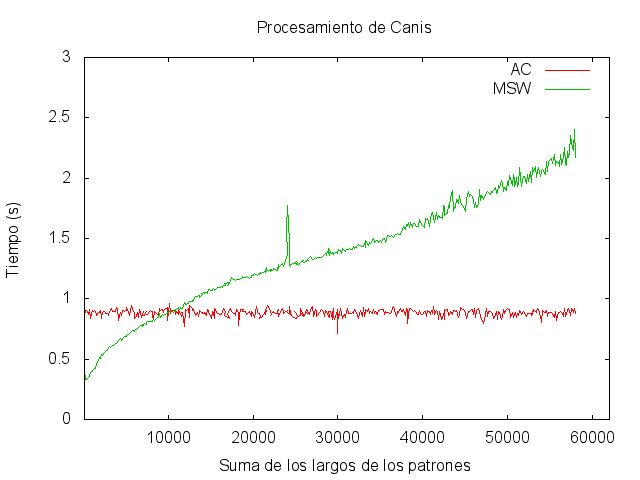
\includegraphics[scale=0.4]{Maci5_10PatsCortos_Canis.png}
	\label{fig:exp2_2Tab_d}}
\caption{Comparación de tiempos entre las pruebas 1, 2, 3 y 4 (medido en Mac)}
\label{fig:exp2_2Tab}
\end{figure}
\subsection{Efecto de los fallos de memoria caché en el rendimiento de los algoritmos}
\label{subsec:falloscache}
Con el fin de comprender estos resultados, se analiza la situación de la memoria caché en la ejecución de ambos algoritmos. Se utilizó el programa $\href{http://valgrind.org/}{Valgrid}$ \footnote{Sitio web de Valgrid - http://valgrind.org/} para simular algunas ejecuciones sobre los juegos de pruebas tres y cuatro. Las simulaciones fueron realizadas en Mac y Ubuntu, los datos presentados en este documento corresponden a las ejecuciones sobre Mac; no obstante, en Ubuntu se obtuvieron similares resultados.\\
Las medidas que se consideran en el análisis son:
\begin{itemize}
\item  {\it Ir} : Número de instrucciones ejecutadas.
\item  {\it Dr} : Número de accesos a caché.
\item  {\it D1 misses} : Número de fallos de lectura + fallos de escritura en el nivel 1 del caché.
\item  {\it LLd misses} : Número de fallos de lectura + fallos de escritura en el último nivel del caché.
\item  {\it D1MR} : La tasa de fallos de caché de nivel 1, la cual se define en \cite{bruce07} como $\frac{D1 misses}{Dr}$
\end{itemize}

\begin{table}[H]
\begin{center}
\scalebox{0.5} {
\begin{tabular}{lllllllllll}
\hline
  Total de caracteres\\ de patrones & \multicolumn{4}{c}{AC} & \multicolumn{4}{c}{MSW}\\

 & Ir & Dr & D1 misses & LLd misses  & D1MR  
 & Ir & Dr & D1 misses & LLd misses & D1MR  \\
  \midrule
152&2,234,416,638&1,100,639,130&1,468,835&1,436,691&	0.1	&1,650,365,936&914,344,784&1,505,777&1,437,163&	0.1\\
7711&2,311,573,313&1,145,950,533&73,772,855&1,451,051&	6.4	&1,659,976,386&918,092,533&109,984,409&1,472,333&	11.9\\
15464&2,312,674,348&1,145,689,265&118,963,702&1,467,023&	10.3	&1,670,302,224&921,759,044&122,377,389&1,516,200&	13.2\\
23168&2,313,449,124&1,145,256,163&140,564,456&1,484,593&	12.2	&1,681,348,889&925,424,216&126,393,101&1,577,561&	13.6\\
31075&2,321,743,241&1,149,328,728&153,739,533&1,505,375&	13.3	&1,689,027,898&928,660,247&128,533,849&1,671,861&	13.8\\
38774&2,326,427,056&1,151,276,154&160,771,680&1,528,210&	13.9	&1,699,780,189&932,164,070&130,134,560&1,876,071&	13.9\\
46293&2,330,888,470&1,153,133,794&166,657,548&1,551,410&	14.4	&1,706,350,880&934,938,423&130,801,571&2,222,245&	13.9\\
54244&2,335,825,040&1,155,214,790&171,046,365&1,583,281&	14.8	&1,717,504,016&938,584,651&132,001,853&2,918,619&	14\\
61981&2,343,747,921&1,159,143,991&175,323,573&1,617,820&	15.1	&1,724,797,823&941,448,518&132,382,025&4,025,800&	14\\
  \bottomrule
\end{tabular} }
\captionof{table}{Datos de caché de la prueba 3 sobre el texto Canis} \label{tab:Prueba1Cache} 
\end{center}
\end{table}

\begin{table}[H]
\begin{center}
\scalebox{0.5} {
\begin{tabular}{lllllllllll}
\hline
  Total de caracteres\\ de patrones & \multicolumn{4}{c}{AC} & \multicolumn{4}{c}{MSW}\\

 & Ir & Dr & D1 misses & LLd misses  & D1MR  
 & Ir & Dr & D1 misses & LLd misses & D1MR  \\
  \midrule
152&2,234,401,677&1,100,635,524&1,468,822&1,436,679&	0.1	&1,650,350,975&914,341,178&1,505,738&1,437,141&	0.1\\
7221&2,218,051,314&1,089,754,707&1,485,822&1,443,909&	0.1	&1,667,205,338&920,557,984&114,142,061&1,472,818&	12.3\\
14474&2,326,341,972&1,153,639,885&1,504,891&1,451,340&	0.1	&1,684,805,417&926,961,265&124,963,029&1,512,145&	13.4\\
21678&2,346,109,041&1,164,412,795&1,515,997&1,458,684&	0.1	&1,702,442,826&933,386,701&128,446,457&1,615,262&	13.7\\
29085&2,337,255,660&1,157,984,784&1,532,988&1,466,148&	0.1	&1,721,099,238&940,044,561&131,244,588&1,866,211&	13.9\\
36284&2,343,421,387&1,160,598,094&1,549,925&1,473,574&	0.1	&1,739,546,344&946,515,236&132,295,339&2,637,328&	13.9\\
43303&2,343,395,748&1,159,522,319&1,562,490&1,480,773&	0.1	&1,757,495,713&952,801,842&133,099,606&4,500,478&	13.9\\
50754&2,282,819,598&1,122,060,519&1,578,185&1,495,522&	0.1	&1,776,786,022&959,530,443&134,493,371&7,875,837&	14.0\\
57991&2,386,121,854&1,182,942,024&1,590,988&1,523,510&	0.1	&1,795,440,485&966,083,880&135,150,380&12,046,266&	13.9\\
  \bottomrule
\end{tabular} }
\captionof{table}{Datos de caché de la prueba 4 sobre el texto Canis} \label{tab:Prueba2Cache} 
\end{center}
\end{table}

Como se muestra en los cuadros \ref{tab:Prueba1Cache} y \ref{tab:Prueba2Cache}, la implementación de la segunda etapa del algoritmo MSW ejecuta siempre menos instrucciones que la de AC. Se puede apreciar que en la situación del cuadro \ref{tab:Prueba1Cache}, ambos algoritmos presentan una tasa similar de fallos de caché de nivel uno, que es creciente con la suma de los largos de los patrones. Esto es consistente con la figura \ref{fig:exp2_2Tab_c}, en la cual los tiempos de ejecución son crecientes tanto para MSW como para AC, estando la curva de MSW siempre por debajo de la de AC.\\
En el cuadro \ref{tab:Prueba2Cache}, en cambio observamos que la tasa de fallos de caché de nivel uno en MSW tiene un comportamiento similar al del cuadro \ref{tab:Prueba1Cache}, pero la tasa de fallos de caché de nivel uno de AC se mantiene constante y nunca supera a la de MSW. Esto es nuevamente consistente con la figura \ref{fig:exp2_2Tab_d}, donde el tiempo de ejecución de AC se mantiene aproximadamente constante. Para instancias suficientemente grandes, el mejor aprovechamiento de la memoria caché termina inclinando la balanza a favor de AC.\\
Otra medida recogida de las pruebas es la cantidad de fallos de memoria caché del último nivel, para MSW, la misma presenta un crecimiento abrupto en las últimas filas de los cuadros \ref{tab:Prueba1Cache} y \ref{tab:Prueba2Cache}, siendo más notorio en el cuadro \ref{tab:Prueba2Cache}. Por su lado, la cantidad de fallos de memoria caché del último nivel de AC no varía de forma considerable en ningún caso.\\
De lo analizado anteriormente y resultados obtenidos en otros experimentos que no se presentan en este documento por arrojar resultados similares a los ya presentados, se puede concluir que los fallos de memoria caché, así como los de página (en memoria principal) redundan negativamente en el rendimiento de los algoritmos presentados. En condiciones en las cuales estos fallos afectan a ambos algoritmos de forma equitativa MSW obtendrá mejores tiempos que AC, sin embargo, para juegos de patrones configurados de forma tal que la estructura de AC obtenga baja tasa de fallos de caché este último algoritmo superará a MSW. En particular, tomando juegos de pruebas con patrones suficientemente largos MSW consumirá una cantidad de memoria que puede llevar a que el sistema produzca más fallos de caché y de página (enlenteciendo la ejecución) comparado con AC.
\subsubsection{Efecto del largo del texto sobre el tiempo de procesamiento de texto}
Una observación pertinente es que a lo largo del procesamiento de los texto, el tiempo de ejecución medido en cada bloque de lectura presenta una variación muy pequeño. Esta afirmación se observa en las gráficas presentadas en la figura \ref{fig:bloques_procesados}, donde el eje Y representa el tiempo de ejecución por bloque del procesamiento sobre el texto {\it HomoSapiens} y el eje X representa la suma de los largos de los patrones. Se ejecutaron once juegos de patrones correspondientes a la prueba 3 (figura \ref{fig:bloque_3}) y prueba 4 (figura \ref{fig:bloque_4}).\\
En cada ejecución se midió el tiempo del procesamiento de cada uno de los 340 bloques, cada uno de aproximadamente 4MB. En estas gráficas se muestra el promedio de los tiempos obtenidos en cada experimento. También se presenta, en cada punto, una barra que representa la desviación estándar en los datos medidos.
\begin{figure}[H]
\centering
	\subfigure[Prueba 3]{%
	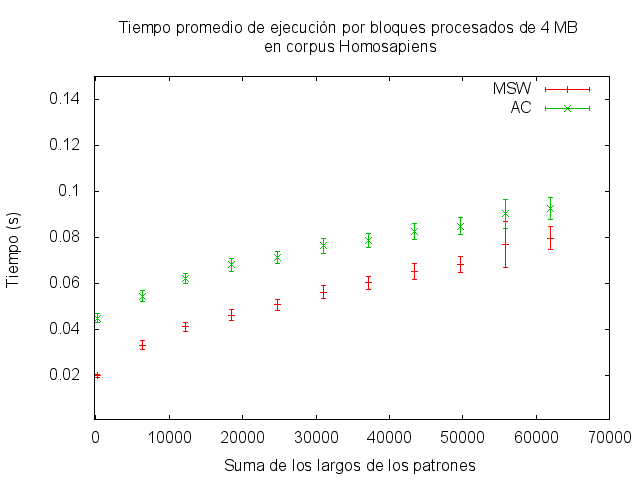
\includegraphics[scale=0.4]{Mac_DesviacionEstandar_Test3.png}
	\label{fig:bloque_3}}
\quad
	\subfigure[Prueba 4]{%
	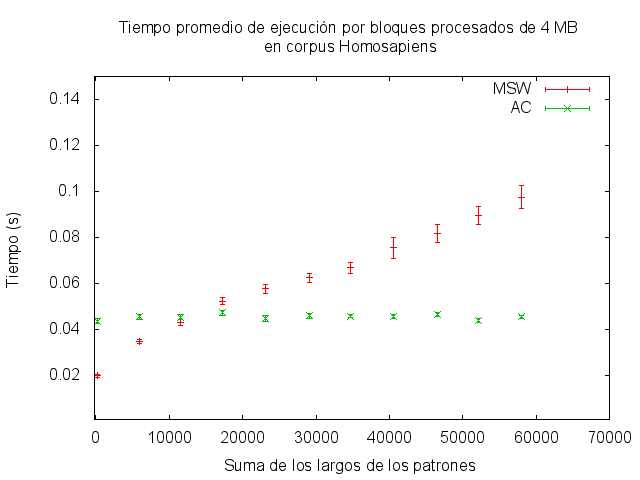
\includegraphics[scale=0.4]{Mac_DesviacionEstandar_Test4.png}
	\label{fig:bloque_4}}
\caption{Tiempo promedio de procesamiento por bloques de lectura (medido en Mac)}
\label{fig:bloques_procesados}
\end{figure}
\section{Tiempo total de ejecución}
En esta sección se presentan los resultados de los tiempos totales de ejecución en las diversas pruebas ejecutadas. 
Para este análisis definimos tiempo total como $t_{f}$ = $t_{pre}$ + $t_{pro}$ + $t_{pos}$, siendo $t_{pre}$ el tiempo de ejecución del pre procesamiento (creación de la estructuras) analizado en la sección \ref{sec:pre_procesamiento}, $t_{pro}$ el tiempo de ejecución del procesamiento del texto (abordado en la sección \ref{sec:procesamiento}) y  $t_{pos}$ el tiempo de post procesamiento. Para el tiempo de post procesamiento no se considera el tiempo de impresión de datos, por lo que, para el algoritmo AC este tiempo es nulo. El algoritmo MSW presenta una fase de post procesamiento, sin embargo pudo comprobarse que la misma es despreciable.\\ 
El tiempo de ejecución total en las pruebas 1 y 2 presentan $t_{pre}$ apreciable. En el caso de las prueba 1, existe un pequeño intervalo en el cual AC presenta ventaja respecto a MSW, luego del cual MSW siempre obtiene mejores tiempos, tanto de procesamiento como totales. Como se ha mencionado anteriormente, el tiempo de pre procesamiento siempre ubica al algoritmo AC con clara ventaja respecto a MSW, sin embargo, en algunas circunstancias, esta ventaja inicial no termina repercutiendo a su favor al recorrer \emph{textos} suficientemente largos. \\
En el cuadro \ref{tab:Total1} se presentan algunos tiempos totales y de procesamiento de la prueba 1. 

\begin{table}[H]
\begin{center}
\scalebox{0.7} {
\begin{tabular}{lllll}
\hline
  Total de caracteres\\ de patrones & \multicolumn{2}{c}{AC} & \multicolumn{2}{c}{MSW}\\

 & $t_{pro}(s)$ & $t_{f}(s)$
 & $t_{pro}(s)$ & $t_{f}(s)$ \\
  \midrule
    284134&42.02&42.11&81.15&81.28\\
    852382&73.64&73.85&107.13&107.51\\
    7952292&197.64&200.03&138.53&142.14\\
    9938725&206.53&209.57&145.75&151.09\\
    14202416&219.86&224.26&159.42&166.09\\
  \bottomrule
\end{tabular}
}
\captionof{table}{Algunos valores de tiempos totales de la prueba 1 sobre el texto HomoSapiens}
\label{tab:Total1} 
\end{center}
\end{table}

El cuadro \ref{tab:Total2} corresponde a algúnos valores tomados en la prueba 2. En dicho cuadro, se muestra en números, la clara ventaja que presenta AC sobre MSW en dicha configuración de prueba.
\begin{table}[H]
\begin{center}
\scalebox{0.7} {
\begin{tabular}{lllll}
\hline
  Total de caracteres\\ de patrones & \multicolumn{2}{c}{AC} & \multicolumn{2}{c}{MSW}\\

 & $t_{pro}(s)$ & $t_{f}(s)$
 & $t_{pro}(s)$ & $t_{f}(s)$ \\
  \midrule
    524912&16.14&16.30&101.01&101.33\\
    2774182&15.49&16.00&123.93&125.85\\
    5274746&16.39&17.35&135.88&139.60\\
    7776769&15.44&16.85&149.97&155.79\\
    10272380&16.76&18.59&160.86&168.80\\
	12777202&16.97&19.26&171.76&181.45\\
  \bottomrule
\end{tabular}
}
\captionof{table}{Algunos valores de tiempos totales de la prueba 2 sobre el texto HomoSapiens}
 \label{tab:Total2}
\end{center}
\end{table}
  
En el cuadro \ref{tab:Total3} se presentan algunos tiempos totales de la prueba 3, como puede apreciarse, MSW mantiene su ventaja respecto de AC. Se observa en ese cuadro que la diferencia entre el tiempo de procesamiento y el tiempo total de ejecución, es decir, $t_{pre}$, es casi despreciable; esto se debe a que la suma de los largos de los patrones que se usaron en la prueba son relativamente pequeños en comparación a los de las muestras utilizadas en las pruebas 1 y 2. De este razonamiento se desprende, y así fue comprobado en pruebas, que los tiempos totales de ejecución de la prueba 4 son equivalentes a los del procesamiento mostrados en la sección \ref{sec:procesamiento}. Por dicho motivo se omitió la presentación de la tabla de tiempos totales de la prueba 4.  
\begin{table}[H]
\begin{center}
 
\scalebox{0.7} {
\begin{tabular}{lllll}
\hline
  Total de caracteres\\ de patrones & \multicolumn{2}{c}{AC} & \multicolumn{2}{c}{MSW}\\

 & $t_{pro}(s)$ & $t_{f}(s)$
 & $t_{pro}(s)$ & $t_{f}(s)$ \\
  \midrule
    152&15.957630&15.957846&6.241849&6.242040\\
    3138&16.600447&16.601562&8.289137&8.290025\\
    4721&17.226274&17.227594&9.458761&9.460374\\
    15464&21.018896&21.021923&14.07945&14.084688\\
    23168&22.973389&22.977644&15.792082&15.797569\\
    38774&25.932629&25.939657&19.634354&19.644133\\
    54244&28.208693&28.217854&22.898829&22.911264\\
    61981&29.803581&29.813734&24.967764&24.982885\\
  \bottomrule
\end{tabular}
}
\captionof{table}{Algunos valores de tiempos totales de la prueba 3 sobre el texto HomoSapiens}
 \label{tab:Total3}
\end{center}
\end{table}
\section{Conclusiones}
En este capítulo se presentó un análisis cuantitativo que muestra las fortalezas y debilidades de los algoritmos en diferentes configuraciones, comparando los tiempos de ejecución obtenidos con las mediciones de consumo de memoria principal y accesos a memoria caché. Se expusieron argumentos que justifican las mediciones obtenidas, presentando conclusiones del rendimiento de los algoritmos que fueron comparados.\\
De las pruebas experimentales surgió que existen diversas configuraciones de datos de entrada que impactan sobre el comportamiento de los algoritmos, de forma tal que en algunos casos MSW presenta mejores tiempos de ejecución (totales y de procesamiento) que AC y vice versa. El algoritmo MSW presenta mejores tiempos cuando el conjunto de patrones a ser buscado es suficientemente grande y el largo de cada patrón es relativamente pequeño. En los casos en que se tengan patrones suficientemente extensos AC presentará mejores tiempos que MSW.\\
También se observó que en todas las configuraciones AC tiene un tiempo de pre procesamiento menor que MSW, pero la diferencia entre estos se puede reducir en la segunda etapa en los casos en que la cantidad de memoria requerida por MSW no afecta negativamente el aprovechamiento de la jerarquía de memoria en mayor medida que AC.
Como trabajo futuro se plantea, dado el análisis de este capítulo, realizar mejoras en las estructuras de datos del algoritmo MSW que permitan reducir los fallos de caché.\\

%Dentro del entregable se encuentran los directorios de experimentación, los cuales contienen los scripts de ejecución de %las pruebas presentadas en este capítulo y otras que no fueron incluidas. También se encuentran los resultados obtenidos %en las ejecuciones en las distintas computadoras.